\documentclass[10pt, a4paper]{scrartcl}

\usepackage{vorschule}
\usepackage[
    typ=ab,
    fach=Informatik,
    lerngruppe={IF-EF},
    nummer=5,
    module={Symbole,Lizenzen},
    seitenzahlen=keine,
    farbig,
    lizenz=cc-by-nc-sa-4,
]{schule}

\usepackage[
	kuerzel=Ngb,
	reihe={Objektorientierte Programmierung},
	version={2019-11-14},
]{ngbschule}

\author{J. Neugebauer}
\title{Wahrheitswerte}
\date{\Heute}

\setzeAufgabentemplate{ngbnormal}

\begin{document}

\ReiheTitel

\subsection*{Wahrheitstafeln}
Trage in der Wahrheitstafeln die Wahrheitswerte \code{true} und \code{false} ein.

\smallskip
\begin{tabularx}{\textwidth}{|c|c|*{5}{X|}} \hline
	\textbf{\code{A}} & \textbf{\code{B}} & \textbf{\code{!A}} &
	\textbf{\code{A \&\& B}} & \textbf{\code{A || B}} &
	\textbf{\code{!A \&\& B}} & \textbf{\code{!A || B}} \\\hline
	\code{true} & \code{true} &&&&& \\\hline
	\code{true} & \code{false} &&&&& \\\hline
	\code{false} & \code{true} &&&&& \\\hline
	\code{false} & \code{false} &&&&& \\\hline
\end{tabularx}

\smallskip
\begin{tabularx}{\textwidth}{|c|c|*{4}{X|}} \hline
	\textbf{\code{A}} & \textbf{\code{B}} & \textbf{\code{!(A \&\& B)}} &
	\textbf{\code{A || !(A \&\& B)}} & \textbf{\code{A || (!A \&\& B)}} &
	\textbf{\code{!A \&\& B}} \\\hline
	\code{true} & \code{true} &&&& \\\hline
	\code{true} & \code{false} &&&& \\\hline
	\code{false} & \code{true} &&&& \\\hline
	\code{false} & \code{false} &&&& \\\hline
\end{tabularx}

\subsection*{Verknüpfte Wahrheitswerte}
Kreuze für die folgenden Testbedingungen an, ob sie in der gegebenen Situation wahr (\code{true}) oder falsch (\code{false}) sind. (Der Rover steht immer auf einem Feld mit Marke, aber ohne Gestein.)

\smallskip
\begin{tabularx}{\textwidth}{|c|X|c|c|} \hline
	\textbf{Situation} & \textbf{Testbedingung} & \textbf{Wahr} &
	\textbf{Falsch} \\\hline
	
	\multirow{4}*{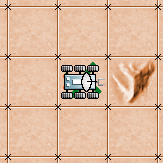
\includegraphics[width=3cm,height=3cm]{EF-AB.5-Abb_Rover1}} &\code{huegelVorhanden("vorne")} &\Zeilenabstand[1cm] & \\\cline{2-4}
	 &\code{!huegelVorhanden("vorne")} &\Zeilenabstand[1cm] & \\\cline{2-4}
	 &\code{gesteinVorhanden() \&\& huegelVorhanden("vorne")} &\Zeilenabstand[1cm] & \\\cline{2-4}
	 &\code{gesteinVorhanden() || !huegelVorhanden("vorne")} &\Zeilenabstand[1cm] & \\\hline

	\multirow{4}*{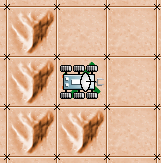
\includegraphics[width=3cm,height=3cm]{EF-AB.5-Abb_Rover2}} &\code{markeVorhanden() \&\& !huegelVorhanden("vorne")} &\Zeilenabstand[1cm] & \\\cline{2-4}
	 &\code{!markeVorhanden() \&\& huegelVorhanden("vorne")} &\Zeilenabstand[1cm] & \\\cline{2-4}
	 &\code{markeVorhanden() \&\& huegelVorhanden("vorne")} &\Zeilenabstand[1cm] & \\\cline{2-4}
	 &\code{markeVorhanden() || huegelVorhanden("vorne")} &\Zeilenabstand[1cm] & \\\hline

	\multirow{4}*{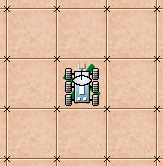
\includegraphics[width=3cm,height=3cm]{EF-AB.5-Abb_Rover3}} &\code{!(!huegelVorhanden("links") \&\& gesteinVorhanden())} &\Zeilenabstand[1cm] & \\\cline{2-4}
	 &\code{(huegelVorhanden("rechts") \&\& !gesteinVorhanden())} &\Zeilenabstand[1cm] & \\\cline{2-4}
	 &\code{markeVorhanden() || (!gesteinVorhanden() \&\& huegelVorhanden("vorne"))} &\Zeilenabstand[1cm] & \\\cline{2-4}
	 &\code{(markeVorhanden() \&\& !gesteinVorhanden()) || (!huegelVorhanden("vorne") \&\& !gesteinVorhanden())} &\Zeilenabstand[1cm] & \\\hline
\end{tabularx}

\end{document}
